\documentclass[12pt]{article}
% packages that I call bc they are in the template I have and I don't know if I want them or not.
\widowpenalty=10000 
\clubpenalty=10000 
\usepackage{amsmath}
\usepackage{amsfonts}
\usepackage{amssymb}
\usepackage{wasysym}
\usepackage{graphicx}
\usepackage{pslatex}
\usepackage{lscape}
\usepackage{rotating}
\usepackage[T1]{fontenc}
\usepackage[latin1]{inputenc}
\usepackage{longtable}
\usepackage[font=scriptsize,labelfont=bf]{caption}
\setlength{\LTcapwidth}{5.5 in}
\usepackage{url}
\usepackage{lastpage}
\usepackage{lineno}
\usepackage[english]{babel}
\usepackage[usenames, dvipsnames]{color}
\usepackage[round, sort, numbers, authoryear]{natbib}
\usepackage{hyperref}
\usepackage{gensymb}
\hypersetup{colorlinks,%
citecolor=black,%
filecolor=black,%
linkcolor=Mahogany,%
urlcolor=MidnightBlue,%
pdftex}

\usepackage{fancyhdr}
\pagestyle{fancy}
 \rhead {\emph{\textcolor{blue}{bgetraer}, \thepage ~of
     \pageref{LastPage}}}

 \lhead{\footnotesize \textsc{GEO~422$/$PSET~4}}
 
 \cfoot{}
 \renewcommand{\headrulewidth}{0.4pt} 





\begin{document}

\section*{Estimation of Earthquake Location and Time}

Using \textit{Geiger's Method}, I created a linearized model of the location and time parameters of the earthquake, such that model parameters adjusted with each iteration to minimize the error between predicted and observed time of seismic wave arrivals. As this linearized model required an initial set of guessed parameters, which could potentially converge to local minima in error rather than the global minimum, I ran the linearized model many times using randomly generated starting parameters. I found the minimum error to be given by the starting parameters $t=19.016$, $x=-48.124$, $y=-158.346$, and $z=118.332$ (see Figure~\ref{fig:stations}). 

\begin{figure}[h!]
\centering
\includegraphics[width=1\textwidth]
{/Users/benjamingetraer/Documents/Fall2017/GEO422/Figures/PSET4/stations.pdf}
\caption[]{Stations are shown as black circles sized by time arrival, estimated location of the earthquake given by minimization of arrival time error is shown as a red triangle.} \label{fig:stations}
\end{figure}
.
\section*{Residuals and Uncertainty}
The uncertainties related to the convergence of \textit{Geiger's Method} were approached by searching for an absolute minimum in error using randomized starting parameters. The minimum error is shown in Figure~\ref{fig:error}, and has a variance ($\approx2$ seconds) smaller than the smallest predicted travel times ($\approx7$ seconds), suggesting that the parameters are close to the global minima.




\begin{figure}[h!]
\centering
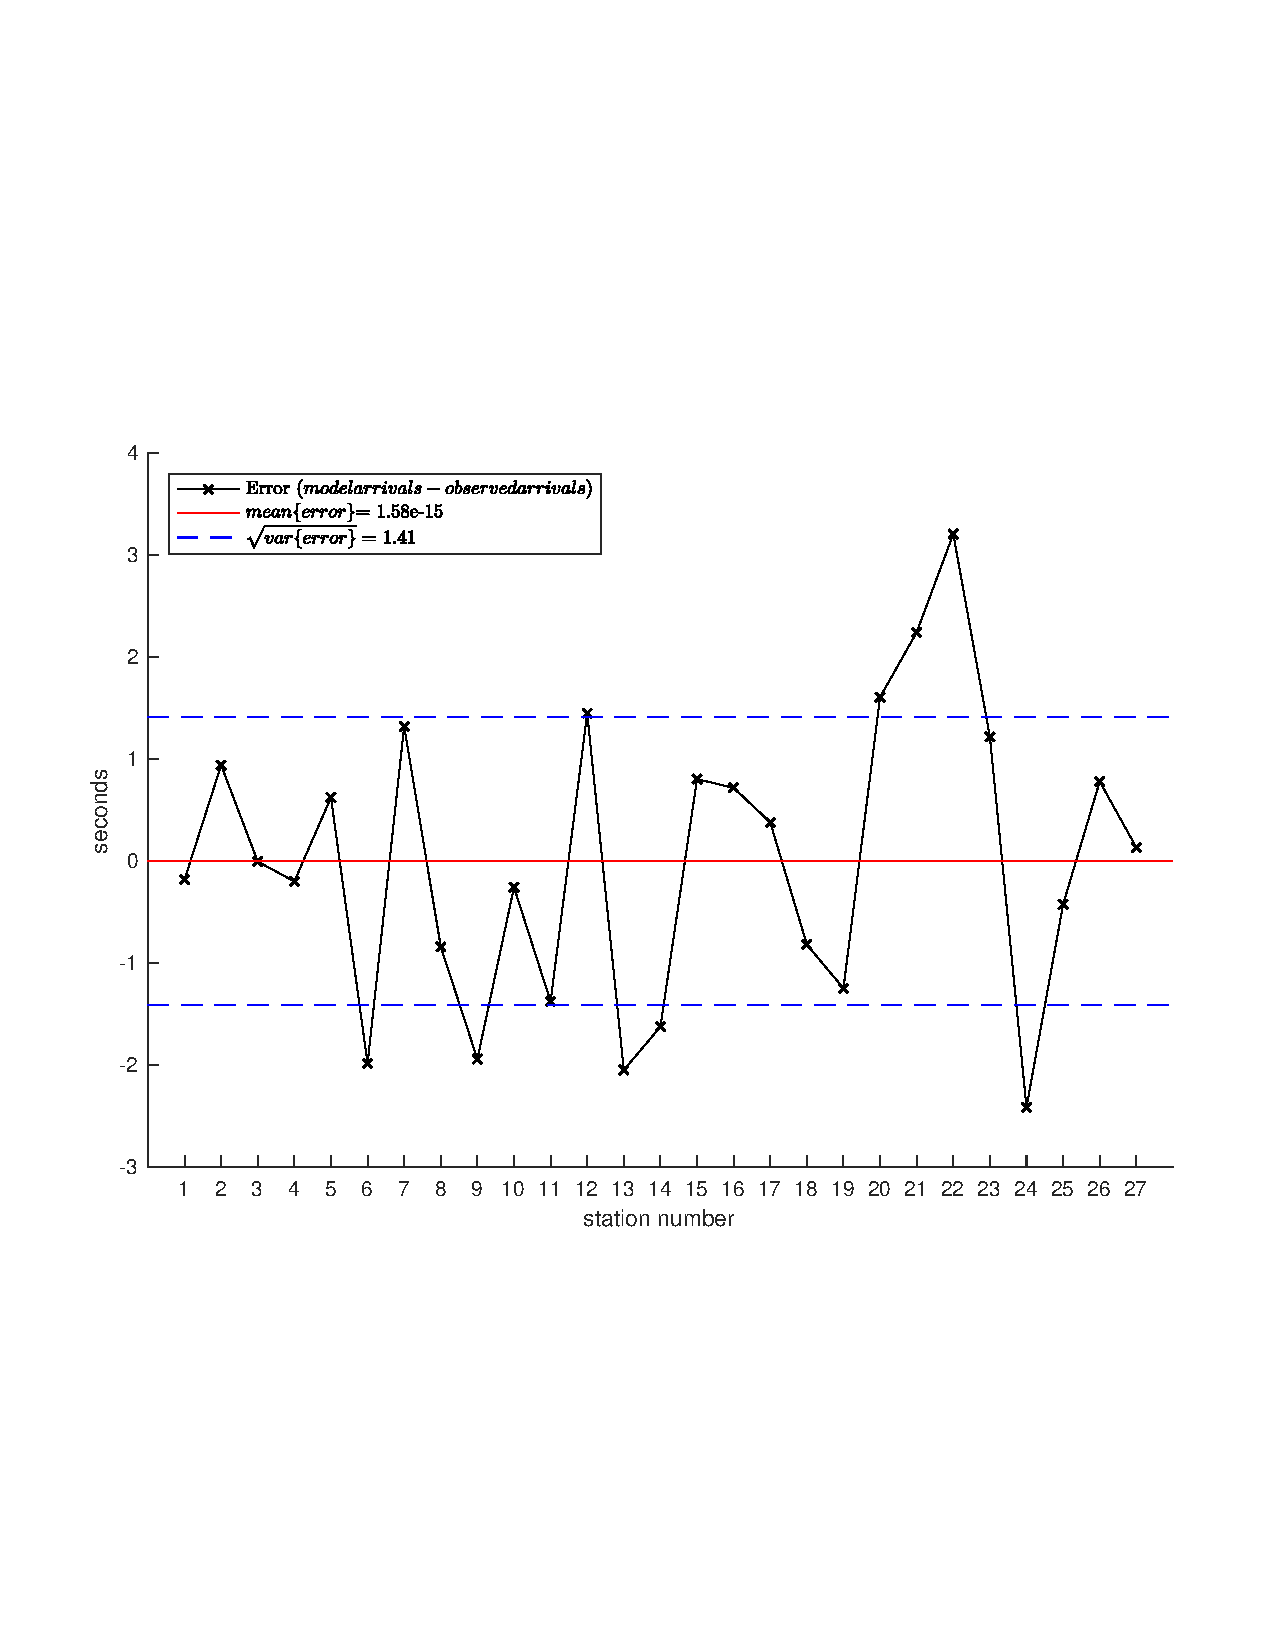
\includegraphics[width=1\textwidth]
{/Users/benjamingetraer/Documents/Fall2017/GEO422/Figures/PSET4/Error.pdf}
\caption[]{The minimized residuals of the predicted arrival times and observed arrival times. Note that the mean is $\approx0$.} \label{fig:error}
\end{figure}




\end{document}


This is never printed
